\documentclass[a4paper,12pt]{article}
\usepackage{graphicx}
\usepackage{caption}
\usepackage{booktabs}
\usepackage{geometry}
\geometry{margin=1in}

\begin{document}

\begin{titlepage}
	\centering

	\huge \textbf{EE 671: VLSI Design} \\
	\vspace{1cm}

	\LARGE \textsc{Course Project 2} \\
	\vspace{4.5cm}

	
\includegraphics[width=0.55\textwidth]{../../icon.png} \\

	\vspace{4.5cm}

	\Large
	\begin{tabular}{rl}
		\textbf{Student Names:}   & Bhuvansh Goyal (22B3908)   \\
		                          & Saarthak Krishan (22B3959) \\
		                          & Hardik Jangir (22B3901)    \\
		                          & Sambhavi Jaiswal (24D0545) \\
		\textbf{Instructor:}      & Prof. Laxmeesha Somappa    \\
		\textbf{Submission Date:} & 28 Nov 2025
	\end{tabular}

	\vfill
\end{titlepage}

\clearpage

\tableofcontents

\clearpage

\section{Introduction}

The Sobel edge detector operates by convolving the input image with two fixed
\(3 \times 3\) kernels: one for the horizontal (\(G_x\)) direction and one for the
vertical (\(G_y\)) direction. The gradient magnitude is then computed from these
two components. While the standard formulation uses the \(L_2\) norm
\(\sqrt{G_x^2 + G_y^2}\), implementing a square root in hardware is expensive.
Therefore, in this design we use the \(L_1\) norm, i.e.,
\(|G_x| + |G_y|\), which is significantly simpler to compute..

Our hardware implementation consists of two main blocks:

\begin{itemize}
	\item \textbf{Valid 3x3 Generator:}
	      This unit continuously streams pixels and produces a valid \(3 \times 3\)
	      window of pixels for each convolution operation.

	\item \textbf{Sobel Core:}
	      This block performs the convolution with the Sobel kernels, computes the
	      gradient magnitude, applies the threshold, and generates the output pixel.
\end{itemize}

The semantics of the key signals are as follows:

\begin{itemize}
	\item \textbf{pixel\_valid:}
	      Input pixels are shifted into the system only when this signal is high.

	\item \textbf{done:}
	      Once all \(256 \times 256\) pixels have been processed, the \texttt{done}
	      signal is asserted. After this point, the module stops producing new
	      outputs and must be reset before processing a new image.

	\item \textbf{threshold\_value} and \textbf{threshold\_wr\_en:}
	      To update the threshold, apply the desired value to \texttt{threshold\_value}
	      and assert \texttt{threshold\_wr\_en}. The Sobel core will then use the new
	      threshold for subsequent output pixels.

	\item \textbf{row\_out} and \textbf{col\_out:}
	      These signals specify the coordinates of the output pixel. The associated
	      \texttt{valid\_out} signal indicates when the output pixel and its
	      coordinates are valid.
\end{itemize}

\begin{figure}[htbp!]
	\centering
	\begin{tabular}{c}
		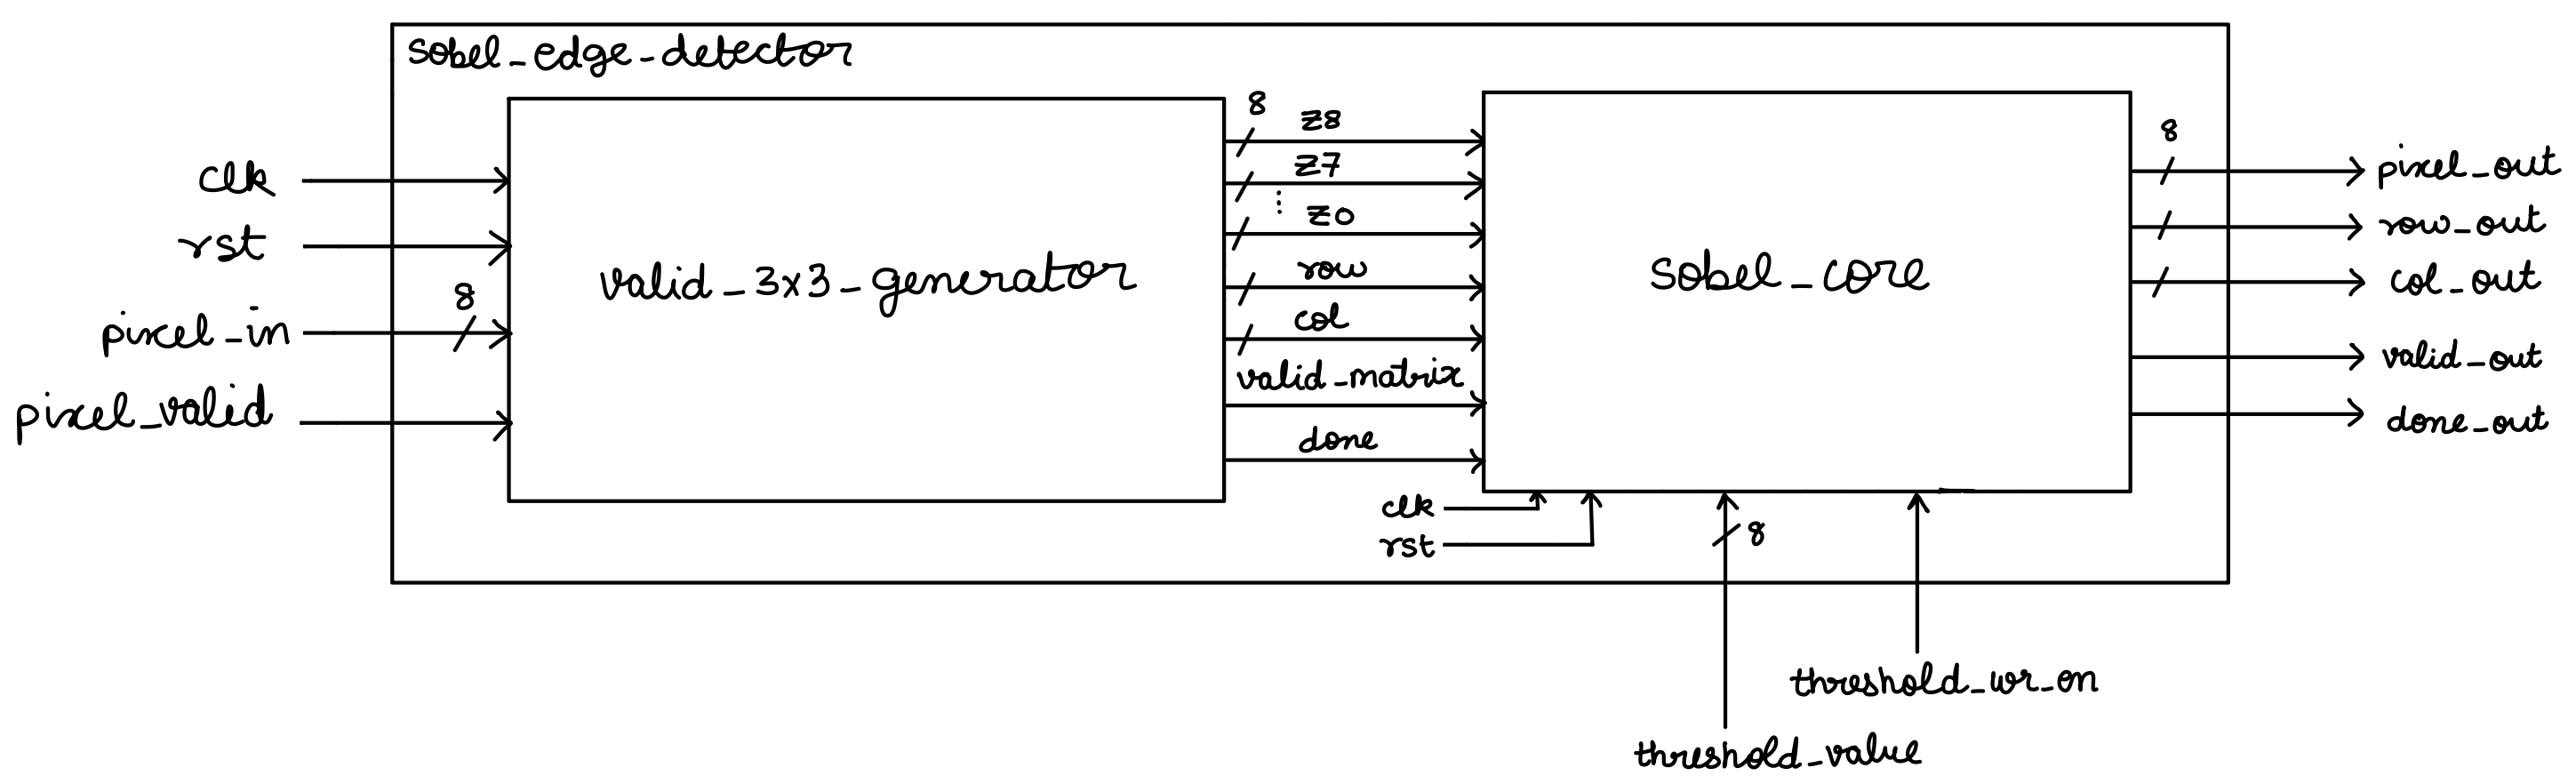
\includegraphics[width=0.9\linewidth]{top_level.png}           \\[6pt]
		(a) Top-level architecture                                     \\[10pt]
		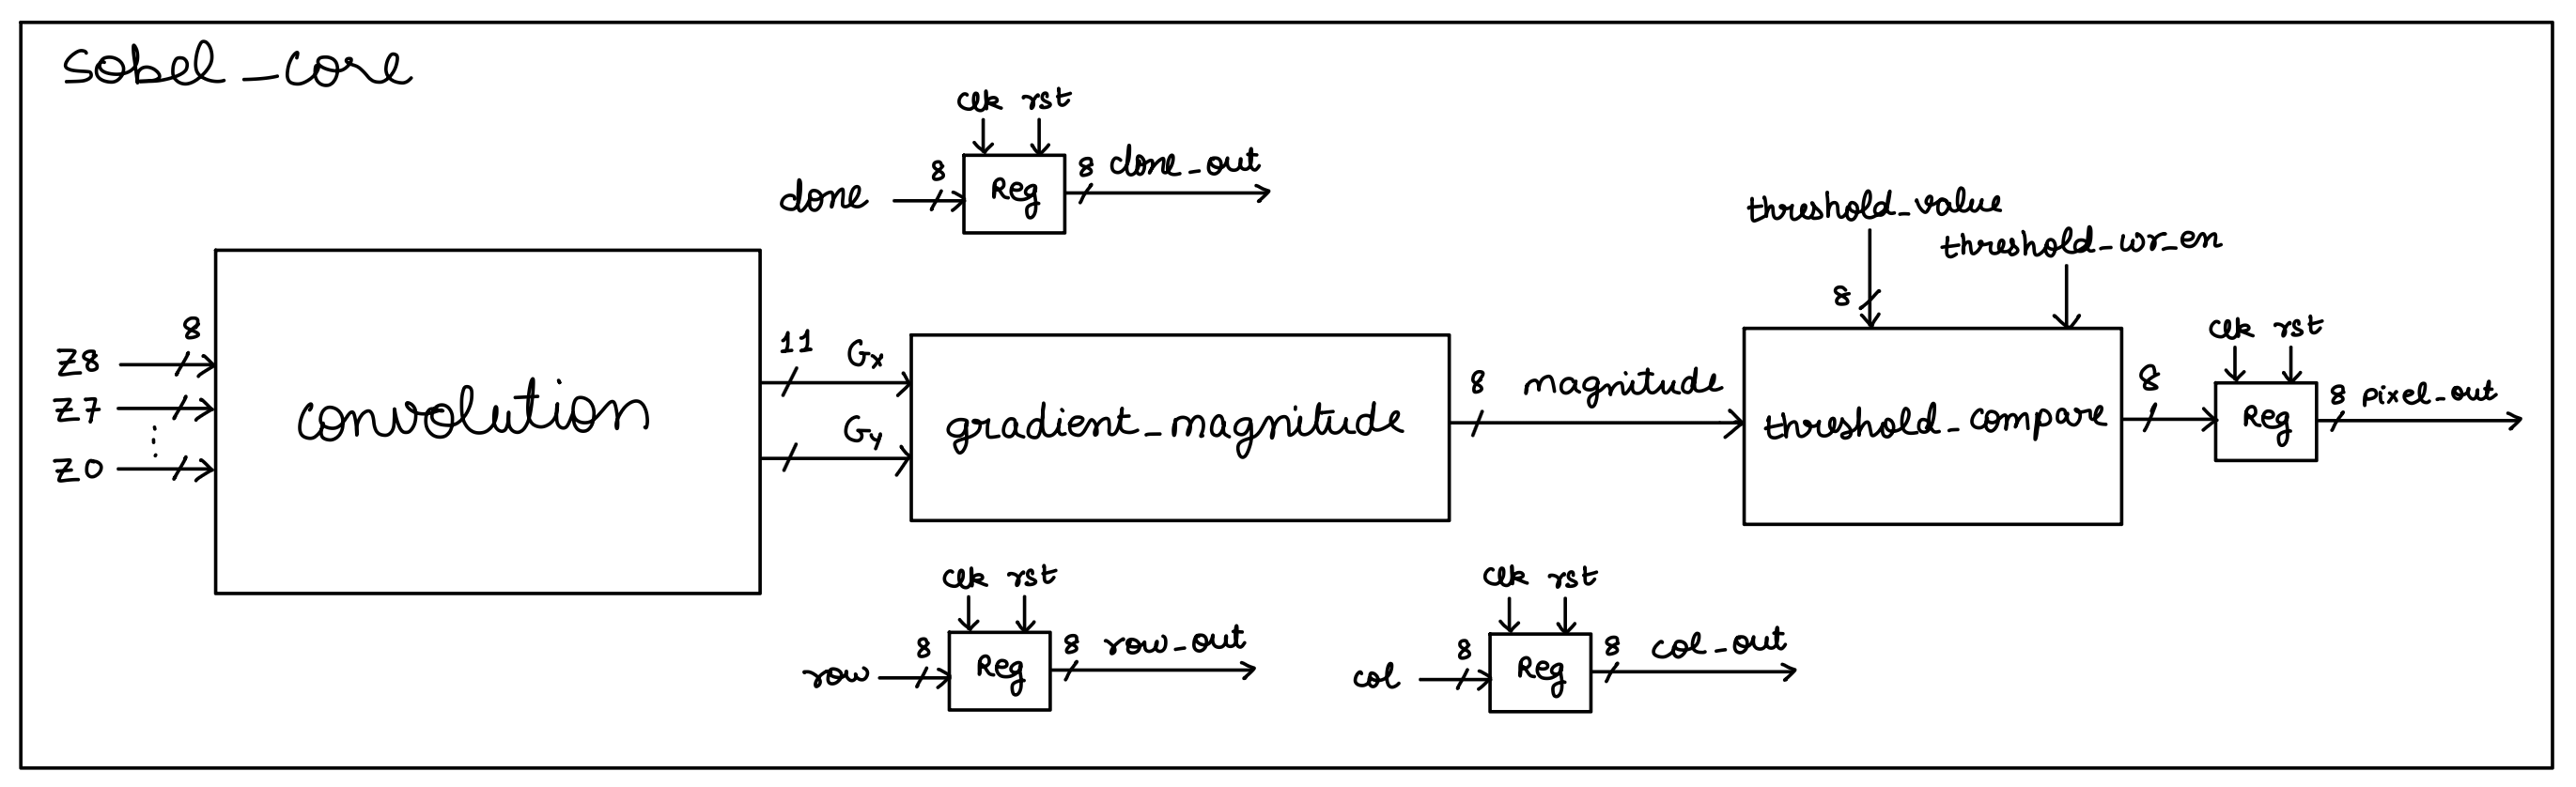
\includegraphics[width=0.9\linewidth]{sobel_core.png}          \\[6pt]
		(b) Sobel core block                                           \\[10pt]
		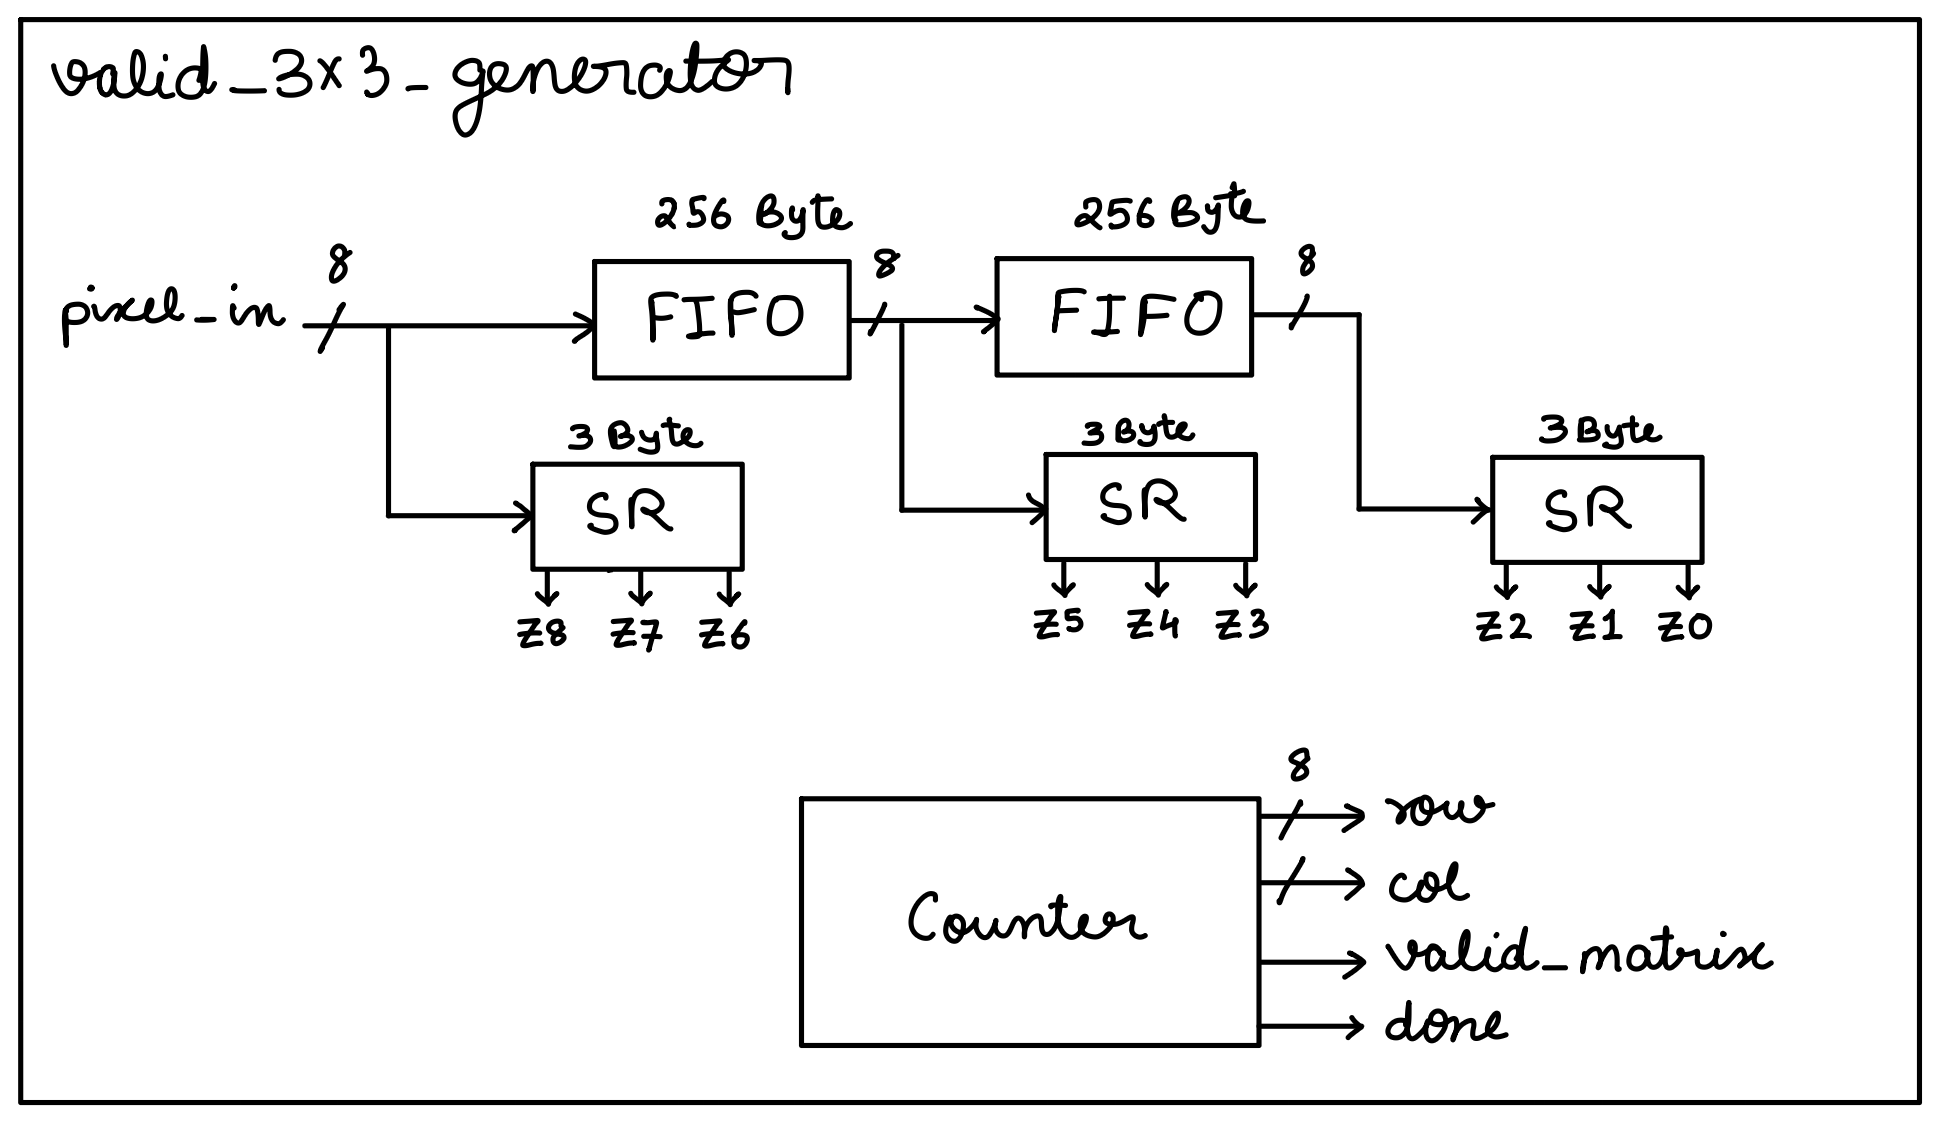
\includegraphics[width=0.9\linewidth]{valid_3x3_generator.png} \\[6pt]
		(c) Valid 3x3 generator
	\end{tabular}
	\caption{Block diagrams of the major components of the Sobel edge detector hardware.}
\end{figure}

\clearpage

\section{Pre-Synthesis Waveform}
\begin{figure}[htbp!]
	\centering
	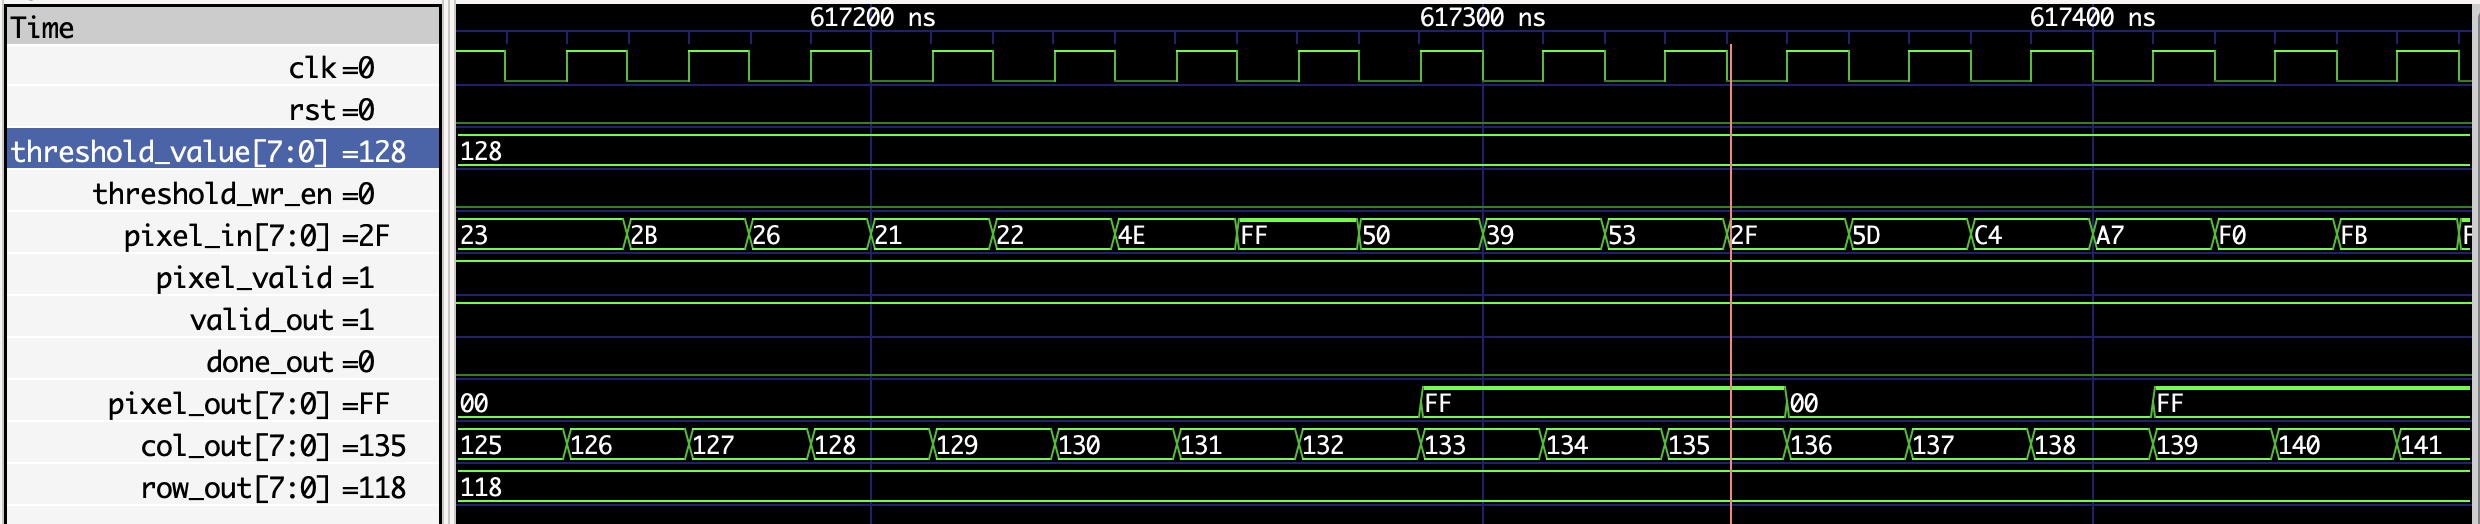
\includegraphics[width=0.95\textwidth]{pre_synthesis_rtl_waveform.png}
	\caption{GTKWave waveform before synthesis}
\end{figure}

\section{Pre-Synthesis Image Output}

\begin{figure}[htbp!]
	\centering
	\begin{tabular}{cc}
		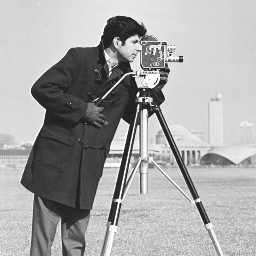
\includegraphics[width=0.38\linewidth]{cameraman.png}                     &
		
\includegraphics[width=0.38\linewidth]{cameraman_output_threshold_128.png}                                \\
		(a) Original Image                                                        & (b) Output at Threshold = 128 \\
		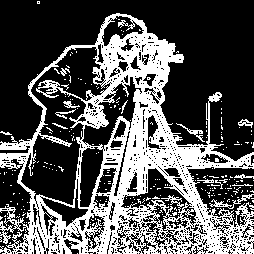
\includegraphics[width=0.38\linewidth]{cameraman_output_threshold_64.png} &
		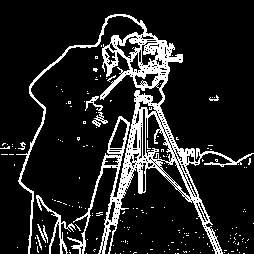
\includegraphics[width=0.38\linewidth]{cameraman_output_threshold_192.png}                                \\
		(c) Output at Threshold = 64                                              & (d) Output at Threshold = 192
	\end{tabular}
	\caption{Pre-synthesis image outputs at various threshold values.}
\end{figure}

\clearpage

\noindent\textbf{Note:}
The testbench reads the input image in hexadecimal format from the \texttt{Images/hex/} directory.
During simulation, it generates an \texttt{output.hex} file at the project root.
To convert this file to a PNG image, navigate to the \texttt{Scripts/} folder and run:

\begin{verbatim}
python hex2img.py
\end{verbatim}

This script uses \texttt{Pillow} and \texttt{NumPy} to convert \texttt{output.hex} into a PNG image placed in the project root.

\section{Synthesis Reports}

\subsection{Area Report}
\begin{figure}[htbp!]
	\centering
	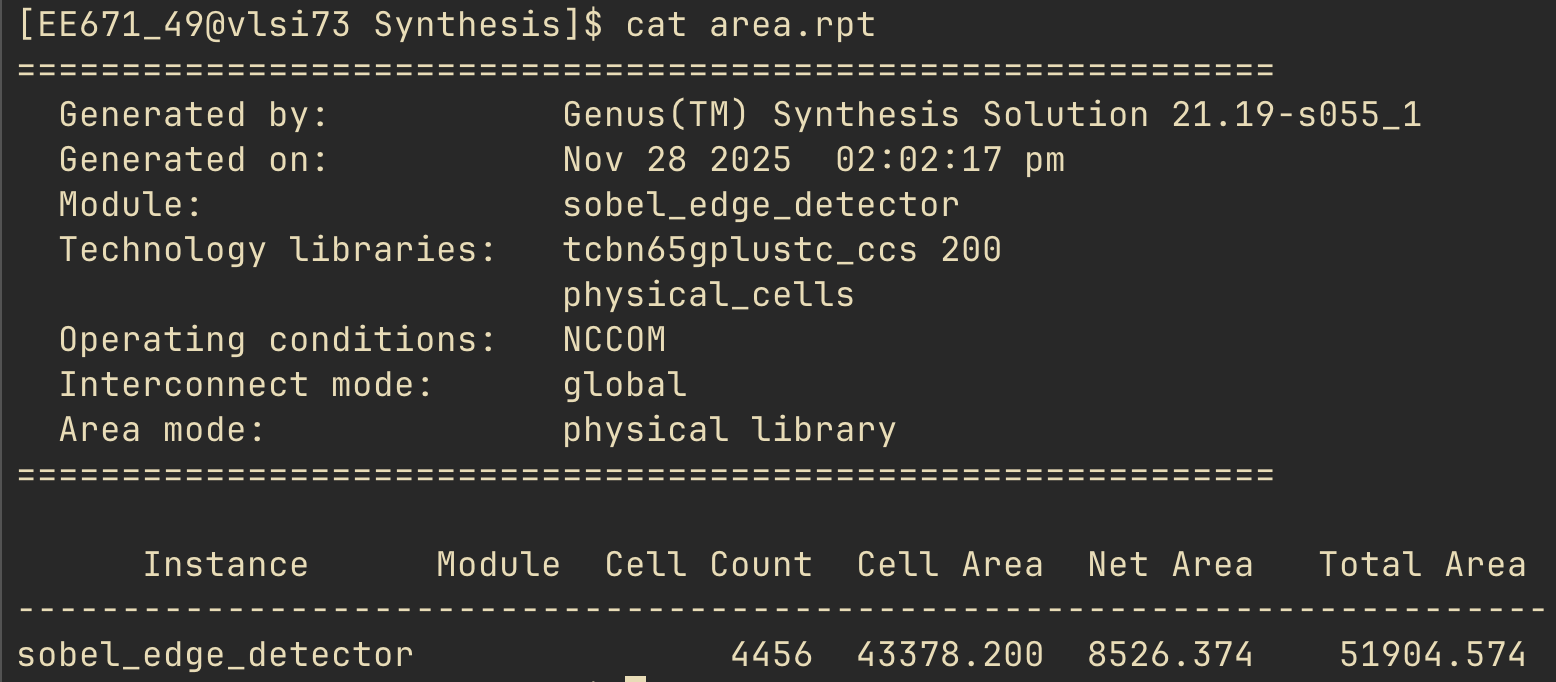
\includegraphics[width=\textwidth]{synthesis_area.png}
	\caption{Area report after synthesis}
\end{figure}

\clearpage

\subsection{Summary Report}
\begin{figure}[htbp!]
	\centering
	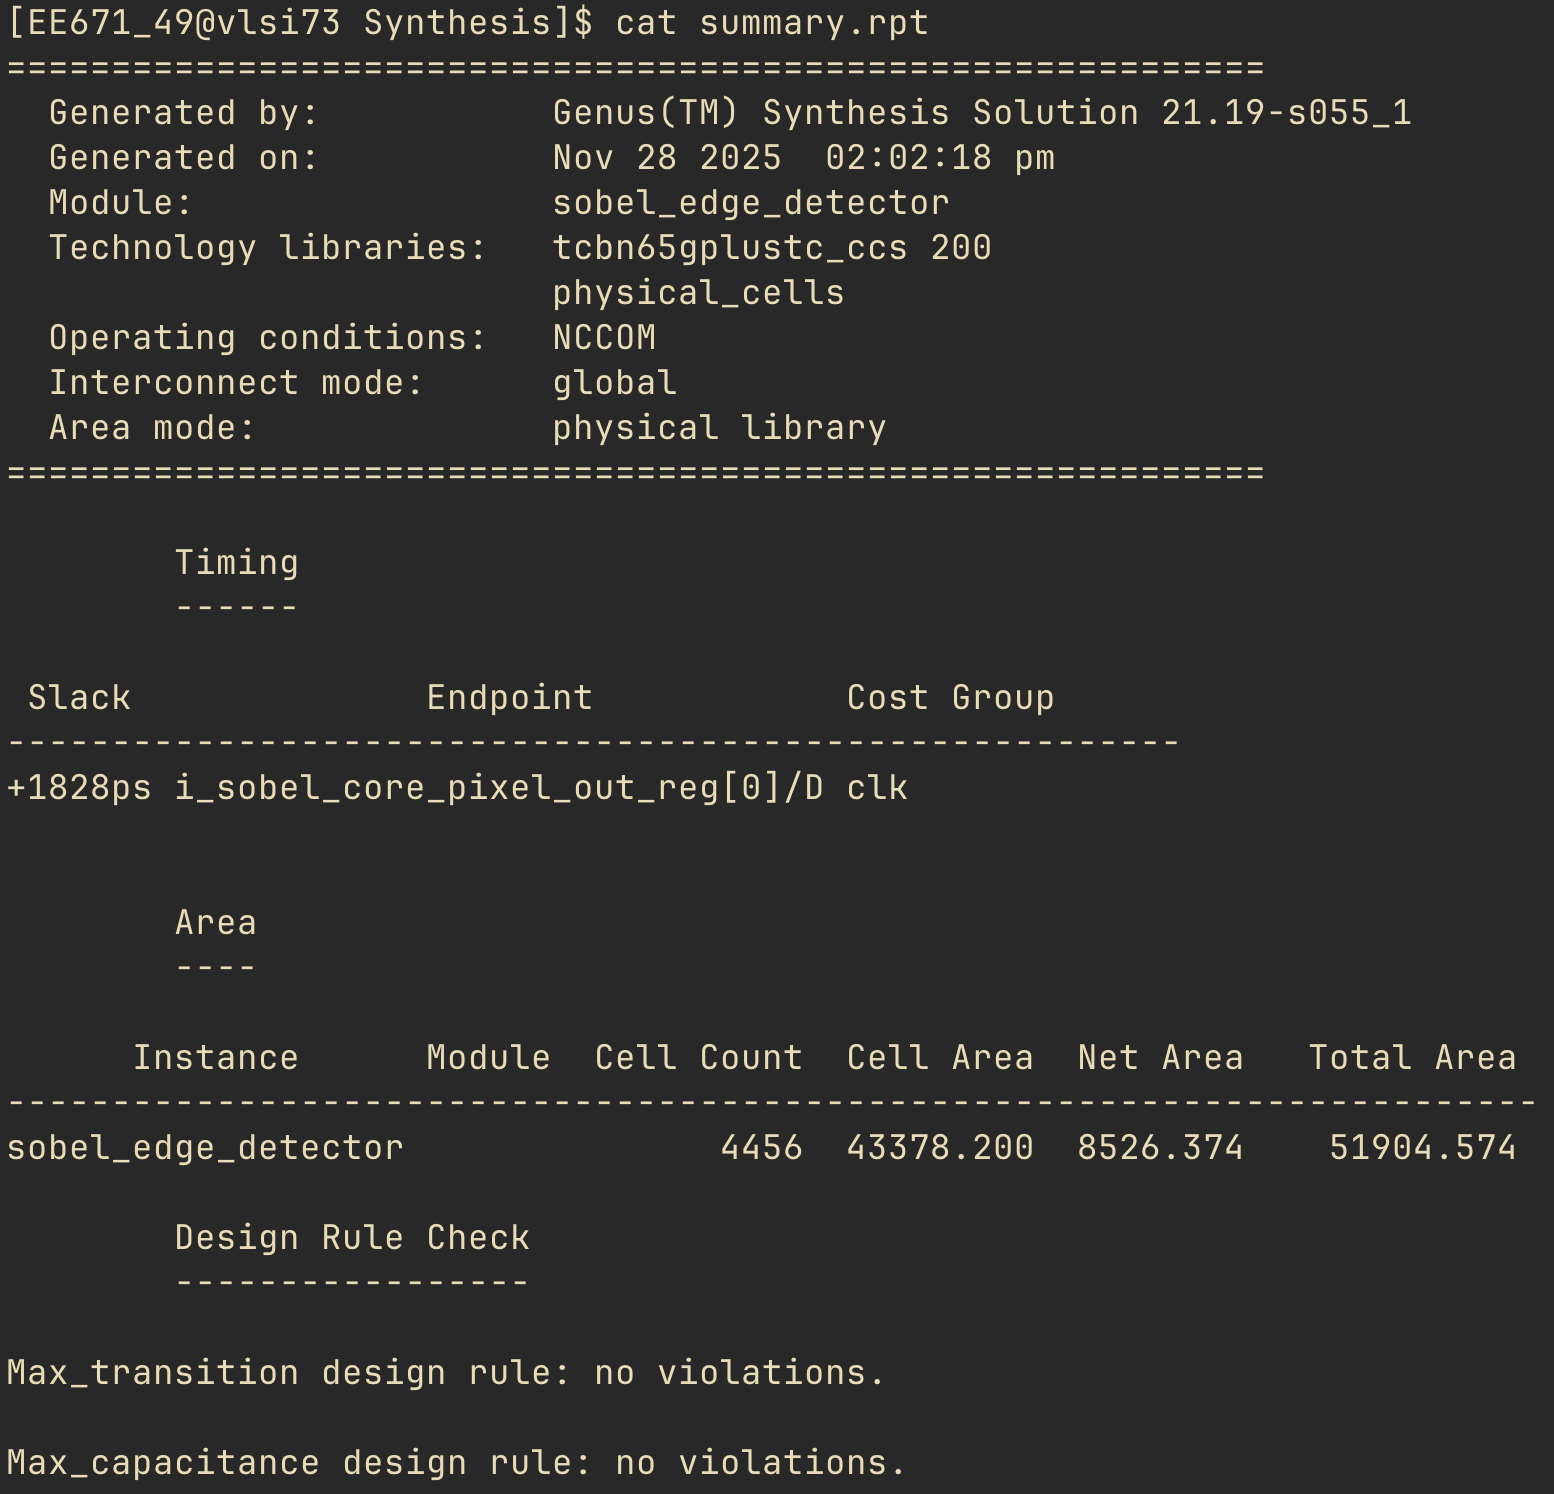
\includegraphics[width=\textwidth]{synthesis_summary.png}
	\caption{Summary report after synthesis}
\end{figure}

\subsection{Cell Count Summary}
\begin{table}[htbp!]
	\centering
	\caption{Cell statistics from RTL synthesis}
	\begin{tabular}{l c}
		\toprule
		\textbf{Parameter}                      & \textbf{Count} \\
		\midrule
		Number of Combinational Cells           & 275            \\[3pt]
		Number of Sequential Cells (Flip-Flops) & 4181           \\[3pt]
		Total Number of Cells                   & 4456           \\[3pt]
		\bottomrule
	\end{tabular}
\end{table}

\section{Post-Synthesis Waveform}
\begin{figure}[htbp!]
	\centering
	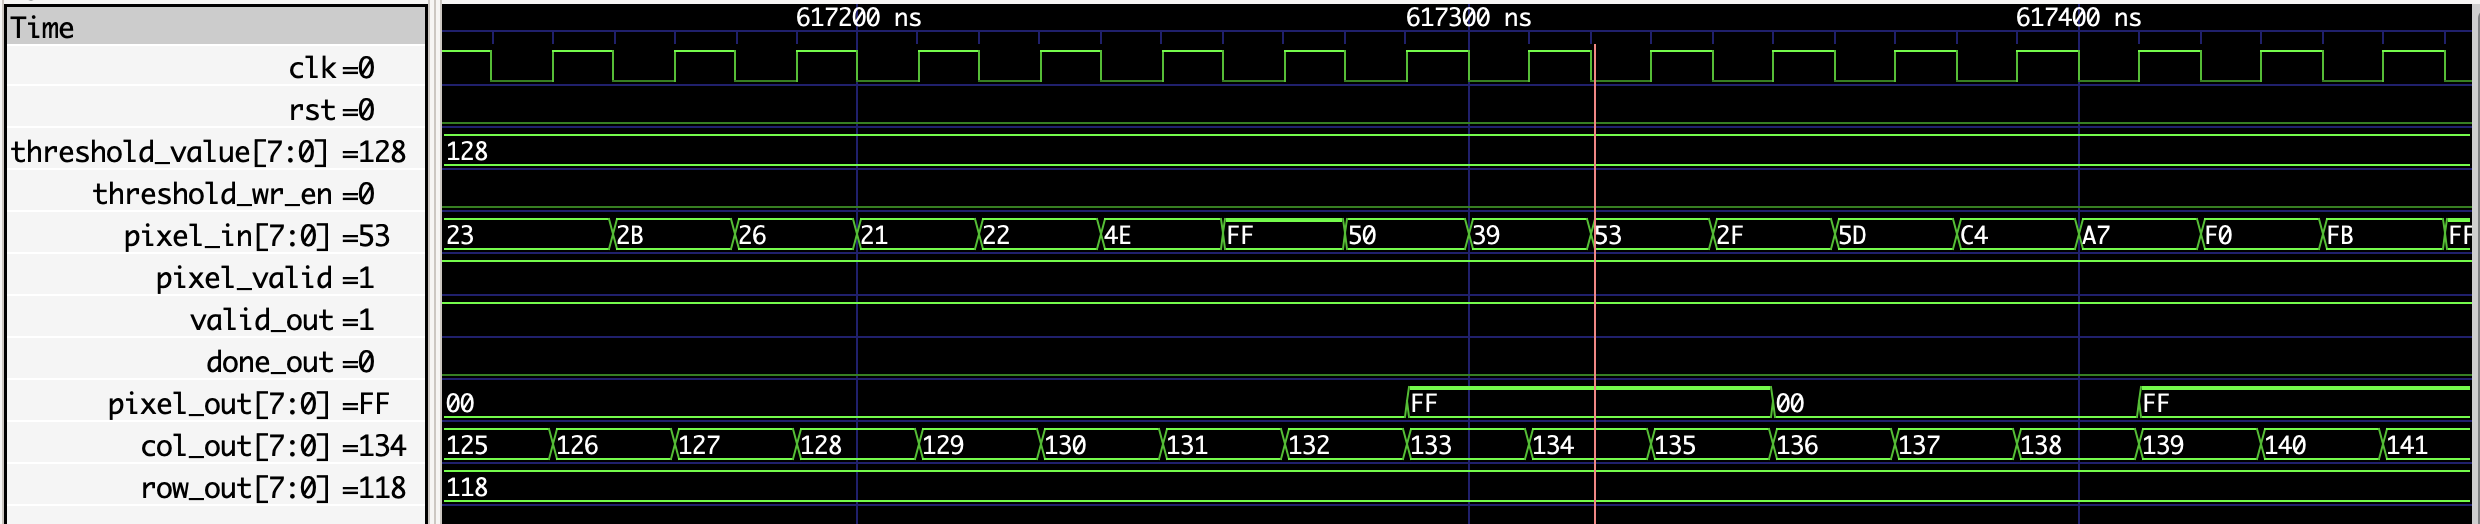
\includegraphics[width=0.95\textwidth]{post_synthesis_rtl_waveform.png}
	\caption{GTKWave waveform after synthesis}
\end{figure}

\section{Post-Synthesis Image Output}

\begin{figure}[htbp!]
	\centering
	\begin{tabular}{cc}
		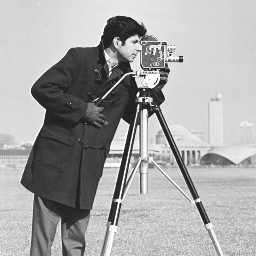
\includegraphics[width=0.38\linewidth]{cameraman.png}                                    &
		
\includegraphics[width=0.38\linewidth]{post_synthesis_cameraman_output_threshold_128.png}                                \\
		(a) Original Image                                                                       & (b) Output at Threshold = 128 \\
		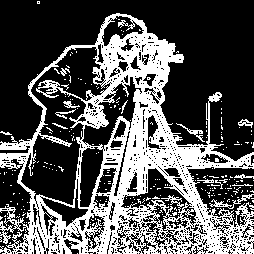
\includegraphics[width=0.38\linewidth]{post_synthesis_cameraman_output_threshold_64.png} &
		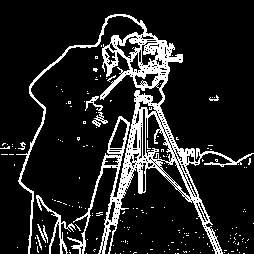
\includegraphics[width=0.38\linewidth]{post_synthesis_cameraman_output_threshold_192.png}                                \\
		(c) Output at Threshold = 64                                                             & (d) Output at Threshold = 192
	\end{tabular}
	\caption{Post-synthesis image outputs at various threshold values.}
\end{figure}

\noindent\textbf{Note:}
The \texttt{output.hex} file generated after running \texttt{./run\_incisive.sh} on the server was copied to the local machine.
The same Python conversion script (\texttt{hex2img.py}) was then executed locally to convert \texttt{output.hex} into a PNG image.

\section{Physical Design Violation Checks}

\subsection{DRC Check}
\begin{figure}[htbp!]
	\centering
	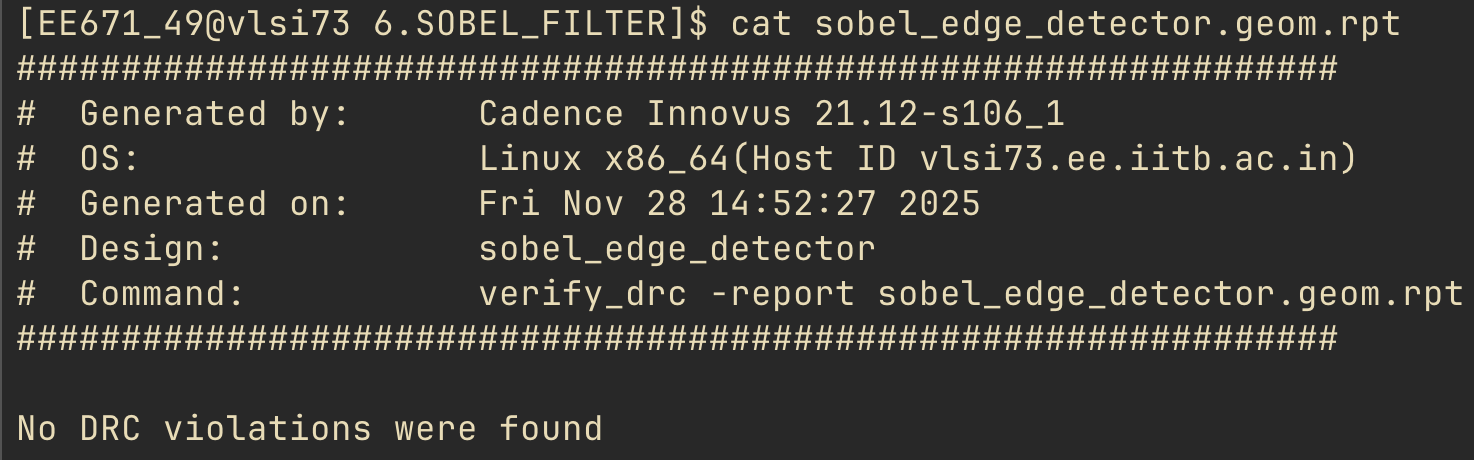
\includegraphics[width=0.95\textwidth]{pnr_drc.png}
	\caption{Design Rule Check (DRC) violations overview}
\end{figure}

\subsection{Antenna Check}
\begin{figure}[htbp!]
	\centering
	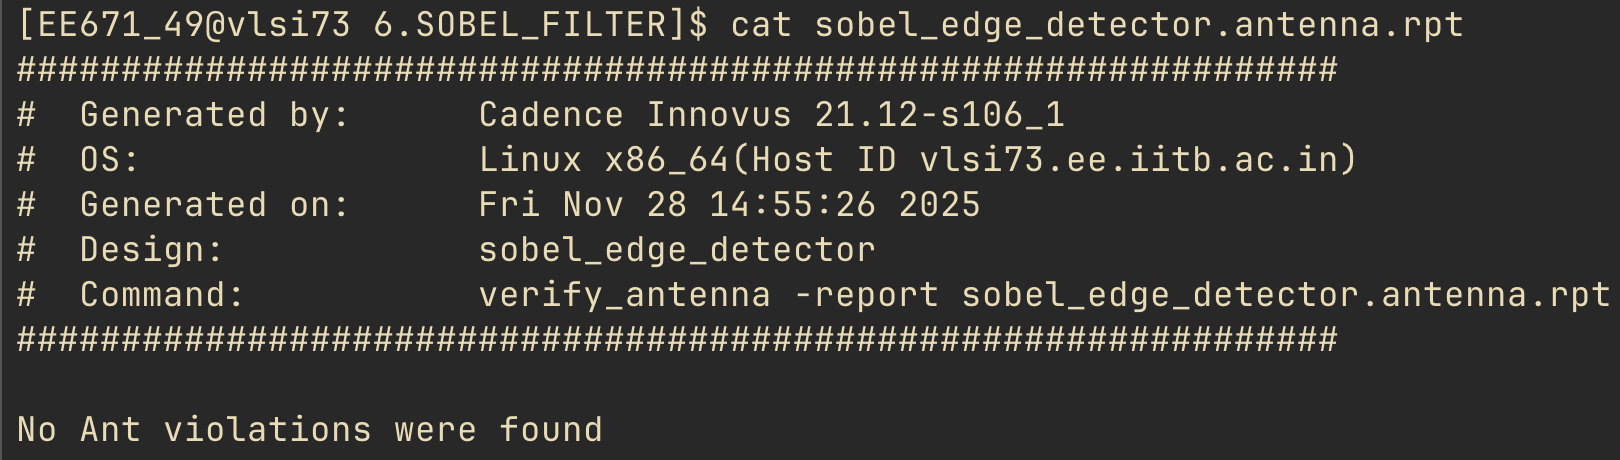
\includegraphics[width=0.95\textwidth]{pnr_antenna.png}
	\caption{Antenna check for the layout}
\end{figure}

\subsection{Connectivity Check}

\begin{figure}[htbp!]
	\centering
	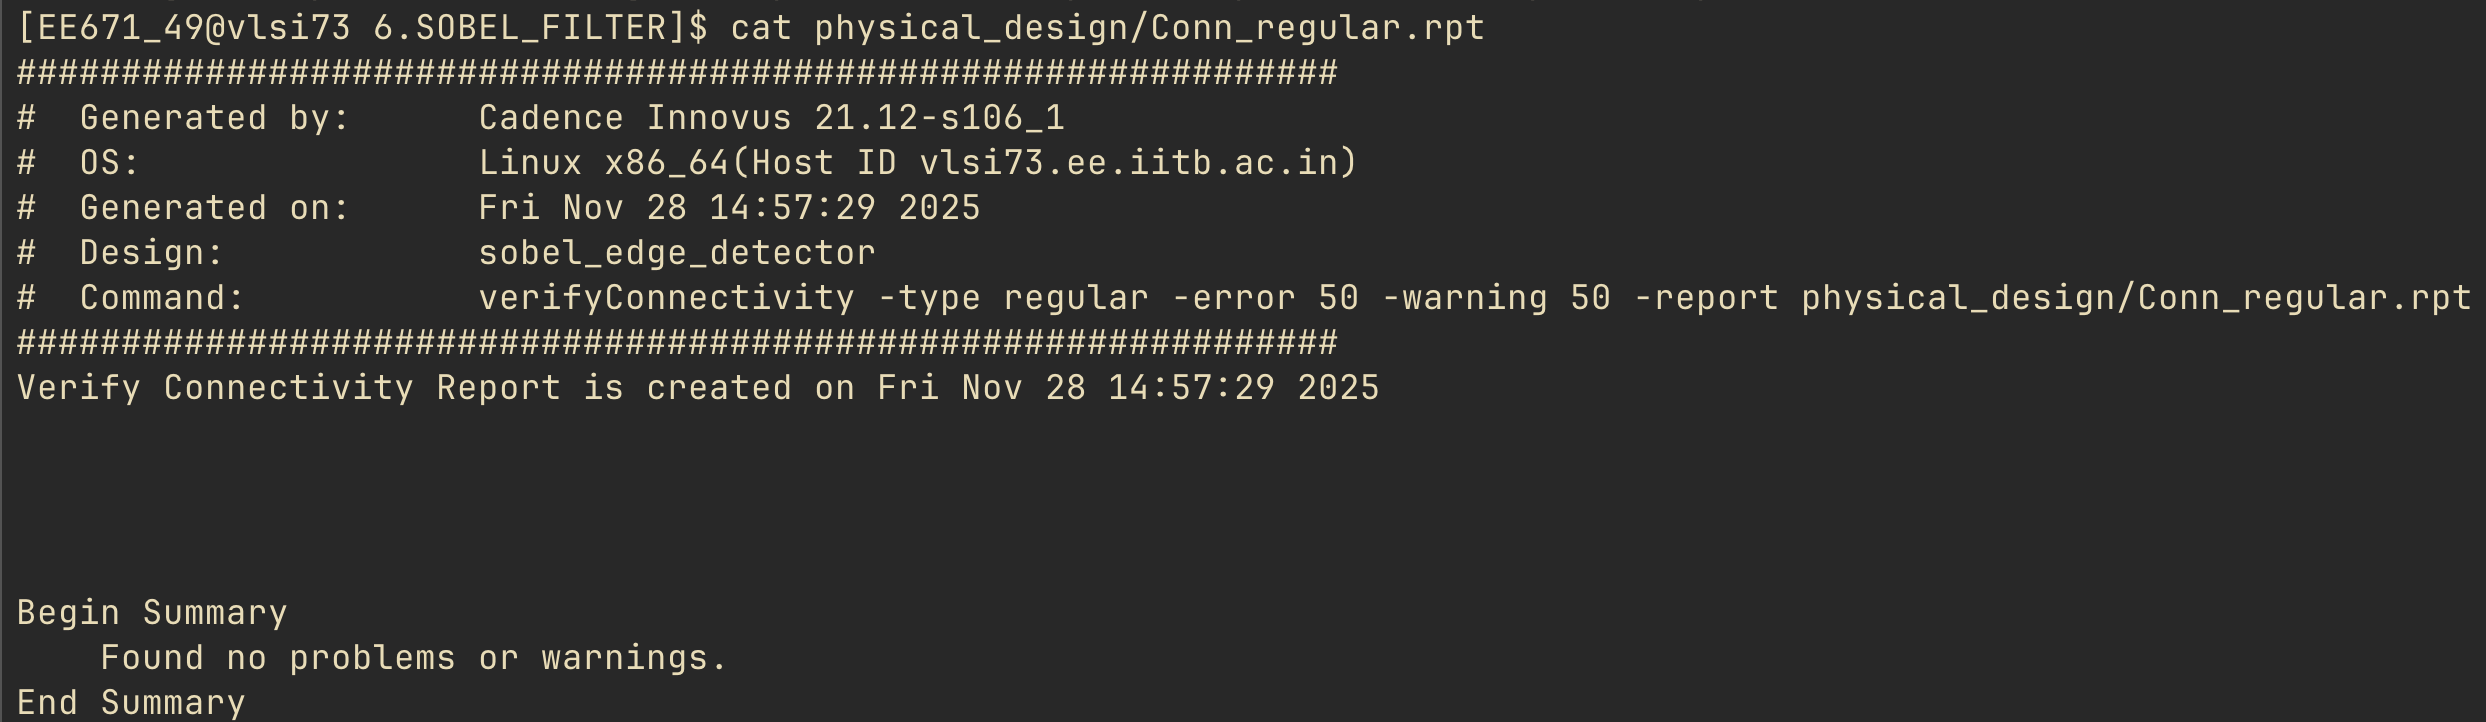
\includegraphics[width=0.95\textwidth]{pnr_connectivity_regular.png}
	\caption{Connectivity check for regular cells}
\end{figure}

\begin{figure}[htbp!]
	\centering
	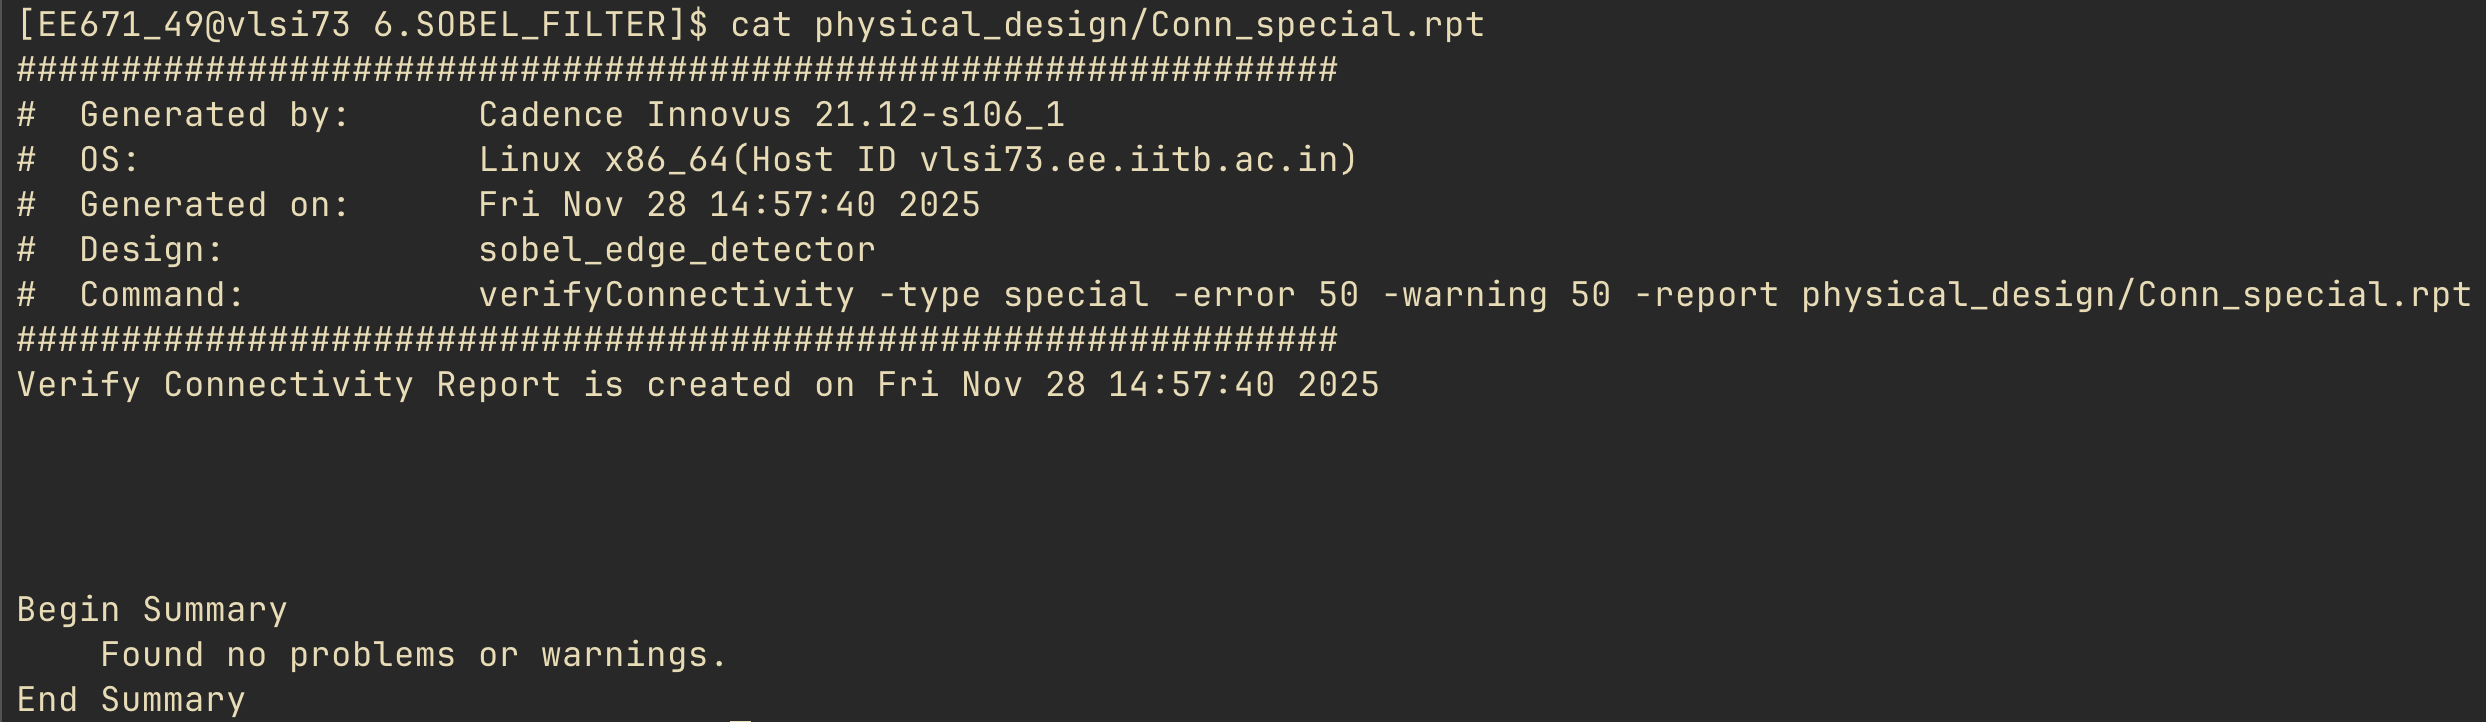
\includegraphics[width=0.95\textwidth]{pnr_connectivity_special.png}
	\caption{Connectivity check for special cells}
\end{figure}

\section{Layout}

\begin{figure}[htbp!]
	\centering
	
\includegraphics[width=0.95\textwidth]{layout.png}
	\caption{Post-route layout of the design}
\end{figure}

\clearpage

\section{Timing, Area and Power Analysis}

\begin{table}[htbp!]
	\centering
	\caption{Post-route Timing, Area, and Power Summary}
	\begin{tabular}{|l|l|}
		\hline
		\textbf{Parameter}                          & \textbf{Value} \\ \hline
		Clock Frequency (MHz)                       & 250            \\ \hline
		Worst Case Setup Slack [WNS] (ns)           & 0.663          \\ \hline
		Worst Case Hold Slack [WNS] (ns)            & 0.015          \\ \hline
		Design Area ($\mu$m$^2$)                    & 51908.40       \\ \hline
		Power Consumption (Sequential Only) (mW)    & 18.84          \\ \hline
		Power Consumption (Combinational Only) (mW) & 1.85           \\ \hline
		Total Power (Internal Only) (mW)            & 19.09          \\ \hline
		Total Power (Switching Only) (mW)           & 2.60           \\ \hline
		Total Power (Leakage Only) (mW)             & 1.46           \\ \hline
		Total Power Consumption (mW)                & 23.15          \\ \hline
	\end{tabular}
\end{table}

\section{Post Physical Design RTL Waveform}

\begin{figure}[htbp!]
	\centering
	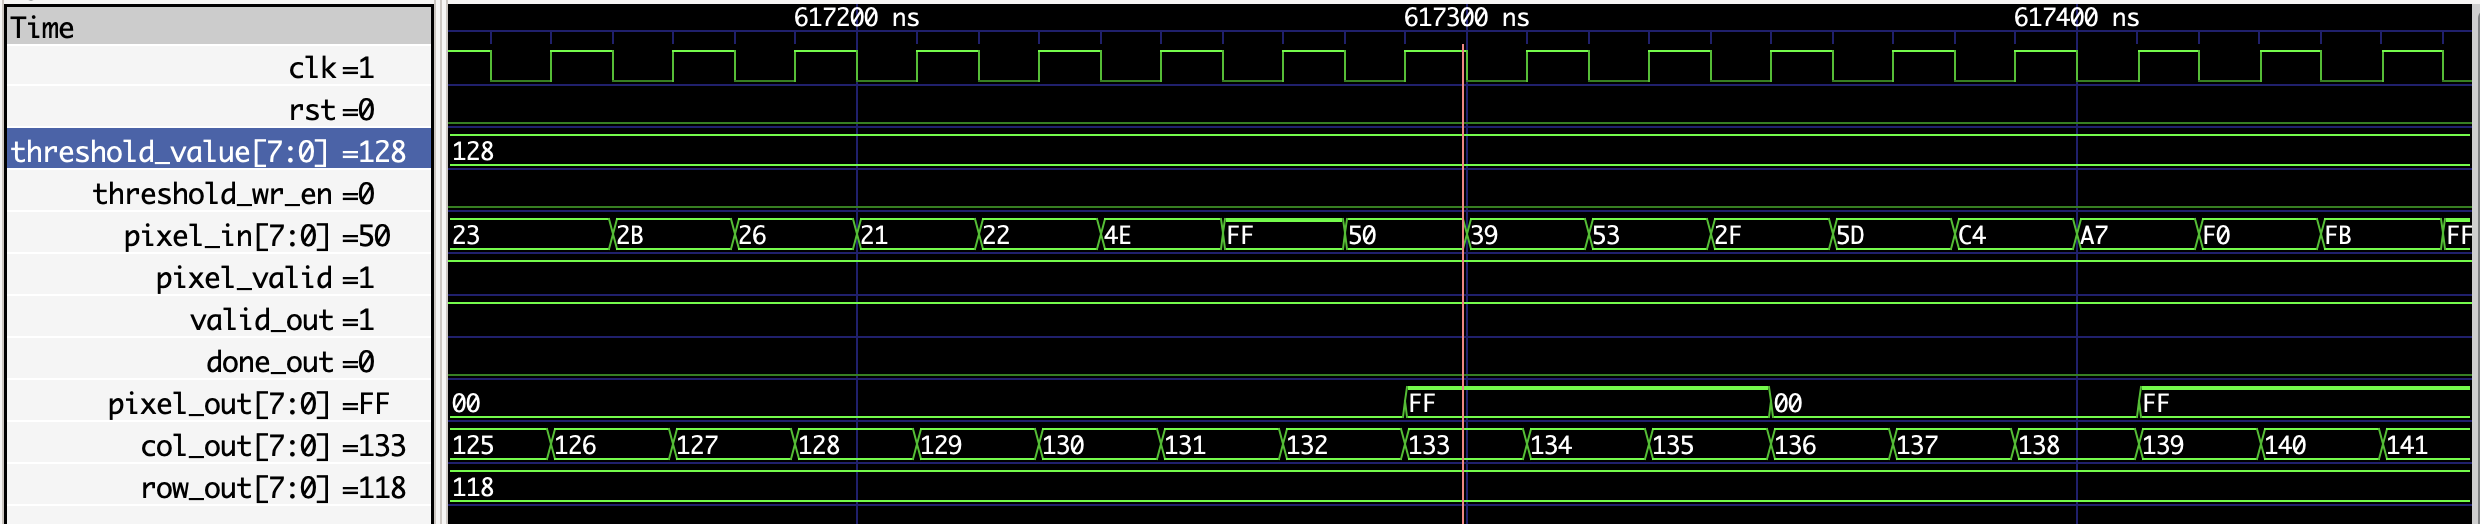
\includegraphics[width=0.95\textwidth]{post_physical_rtl_waveform.png}
	\caption{RTL waveform after physical design}
\end{figure}

\clearpage

\section{Post Physical Design Image Output}

\begin{figure}[htbp!]
	\centering
	\begin{tabular}{cc}
		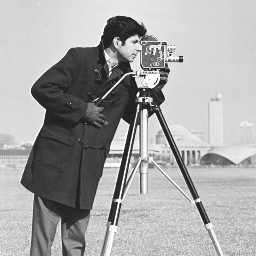
\includegraphics[width=0.38\linewidth]{cameraman.png}                                          &
		
\includegraphics[width=0.38\linewidth]{post_physical_design_cameraman_output_threshold_128.png}                                \\
		(a) Original Image                                                                             & (b) Output at Threshold = 128 \\
		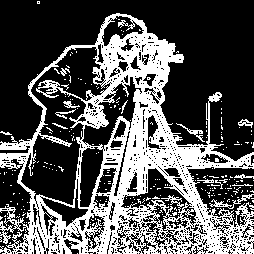
\includegraphics[width=0.38\linewidth]{post_physical_design_cameraman_output_threshold_64.png} &
		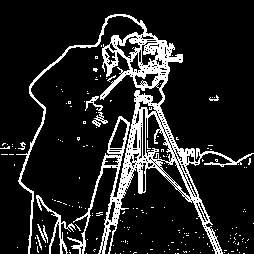
\includegraphics[width=0.38\linewidth]{post_physical_design_cameraman_output_threshold_192.png}                                \\
		(c) Output at Threshold = 64                                                                   & (d) Output at Threshold = 192
	\end{tabular}
	\caption{Post physical design image outputs at various threshold values.}
\end{figure}

\noindent\textbf{Note:}
The \texttt{output.hex} file generated after running \texttt{./run\_incisive.sh} on the server was copied to the local machine.
The same Python conversion script (\texttt{hex2img.py}) was then executed locally to convert \texttt{output.hex} into a PNG image.

\end{document}
